%!TEX root = ./main.tex
\newpage
\section{Problem statement}

\subsection{Dataset presentation}

The data we analysed consists of \textbf{yearly} measurements of \textbf{production} and \textbf{consumption} of \textbf{dairy products} in the \textbf{USA}.

There is a wide range of variables available:

\begin{table}[H]
  \centering
  \begin{tabular}{p{6cm}p{7cm}}
    \toprule
    \multicolumn{2}{c}{\textbf{Production}} \\
    \midrule
    \textbf{Variable}                              & \textbf{Description}                                     \\
    \midrule
    avg\_price\_milk                      & Milk price [\$/lbs]                             \\
    avg\_milk\_cow\_number                & Number of milk cows                             \\
    milk\_per\_cow                        & Milk production [lbs]                           \\
    milk\_production\_lbs                 & Average milk production per cow [lbs/cow]       \\
    milk\_cow\_cost\_per\_animal          & Average cost of a milk cow [\$/cow]             \\
    dairy\_ration                         & Average price for feed rations [\$/lbs]         \\
    alfalfa\_hay\_price                   & Hay price [\$/ton]                              \\
    milk\_feed\_price\_ratio              & Ratio of average price of milk per feed ration  \\
    slaughter\_cow\_price                 & Slaughter cow price [\$/lbs]                    \\
    milk\_volume\_to\_buy\_cow\_in\_lbs   & Milk volume required to purchase a cow [lbs]    \\
    \bottomrule
    \end{tabular}
\end{table}

%\begin{table}[H]
    %\centering
    \begin{longtable}{p{6cm}p{7cm}}
    \toprule
    \multicolumn{2}{c}{\textbf{Consumption [lbs/person]}} \\
    \midrule
    \textbf{Variable}                              & \textbf{Description}                                     \\
    \midrule
    fluid\_milk                           & Milk                                            \\
    fluid\_yogurt                         & Yogurt                                          \\
    butter                                & Butter                                          \\
    cheese\_american                      & American cheese                                 \\
    cheese\_other                         & ``Other cheese''                                 \\
    cheese\_cottage                       & Cottage cheese                                  \\
    Cheddar                               & Cheddar                                         \\
    American.Other                        & Other American cheese                           \\
    Mozzarella                            & Mozzarella                                      \\
    Italian.other                         & Other Italian cheese                            \\
    Swiss                                 & Swiss cheese                                    \\
    Brick                                 & Brick                                           \\
    Muenster                              & Muenster                                        \\
    Cream.and.Neufchatel                  & Cream and Neufchatel                            \\
    Blue                                  & Blue
    \\
    Other.Dairy.Cheese                    & Other dairy cheese                              \\
    Processed.Cheese                      & Processed cheese                                \\
    Foods.and.spreads                     & Foods and spreads                               \\
    \midrule
    evap\_cnd\_canned\_whole\_milk        & Evaporated and canned whole milk                \\
    evap\_cnd\_bulk\_whole\_milk          & Evaporated and canned bulk whole milk           \\
    evap\_cnd\_bulk\_and\_can\_skim\_milk & Evaporated and canned bulk and skim milk \\
    \midrule
    frozen\_ice\_cream\_regular           & Regular frozen ice cream                        \\
    frozen\_ice\_cream\_reduced\_fat      & Reduced fat frozen ice cream                    \\
    frozen\_sherbet                       & Frozen sherbet                                  \\
    frozen\_other                         & Other frozen milk product                       \\
    \midrule
    dry\_whole\_milk                      & Dry whole milk                                  \\
    dry\_nonfat\_milk                     & Dry nonfat milk                                 \\
    dry\_buttermilk                       & Dry buttermilk                                  \\
    dry\_whey                             & Dry whey (milk protein)                         \\
    \bottomrule
  \end{longtable}
%\end{table}

The data provided by \cite{dataset} only covered the period 1980-2014 but we were able to gather the remaining part up until 2021 through the official \textbf{United States Department of Agriculture (USDA)} database. A consistency check was performed to verify the reliability of the newly retrieved data, obtaining values from 2010 to 2014 with the same process and comparing them with the previous source.

At last, we accounted for inflation by adjusting all prices, which allowed us to make meaningful comparisons of prices over time and avoid attributing changes in price only to inflation.

For the spatial analysis section of this report, the data provided by \cite{spatial_data} allowed us to have spatial data regarding the number of cows bred, the amount of cheese and milk sold, and the population of most of the USA counties in 2007 \cite{spatial_data_population}. For lack of data, we decided to take into consideration only the continental USA, without taking into consideration Alaska and Hawaii. At last, to avoid any scalability problems, we logged the variables to proceed with the analysis. 

\subsection{Stakeholder analysis}

To ensure that this report is effective in meeting its intended purpose, it is important to consider the perspectives and needs of the various stakeholders who will be affected by the findings. Therefore, in addition to presenting the data, a stakeholder analysis will also be performed to identify and evaluate the different stakeholders, their interests, and their level of influence. 


A \textbf{power interest matrix} is a visual tool used to analyse stakeholders and their levels of power and interest. The matrix is divided into four quadrants that categorize stakeholders based on their level of power and interest. 
\begin{itemize}
    \item The stakeholders with high power and high interest are placed in the top right quadrant, indicating that they are critical to the success of the project and need to be managed closely. In our case, they are the \textbf{cheese} factories to which this analysis is mainly addressed. 
    \item Those with high power but low interest are placed in the top left quadrant, indicating that they need to be \textbf{kept informed} but may not need to be involved in the details of the project. We identified these criteria with the United States Department of Agriculture (USDA) which is responsible for developing and executing federal laws related to farming. 
    \item Stakeholders with low power but high interest are placed in the bottom right quadrant, indicating that they should be \textbf{kept satisfied} but may not have much influence over the project. These are companies that sell dairy products to consumers through grocery stores, supermarkets, and other outlets.
    \item Finally, stakeholders with low power and low interest are placed in the bottom left quadrant, indicating that they require \textbf{minimal effort} to manage. These are the end users of dairy products. They are impacted by changes in milk prices and market conditions. However, it's not their main concern, nor do they have decisional power.
\end{itemize}

\fg[Power interest matrix.]{0.85}{report-power-interest-matrix.pdf}

\subsection{Research question}
Following the stakeholder analysis, we structured our project over a case study concerning a high-power, high-interest stakeholder: a new dairy producer.\\
The analysis aims at answering the following research questions: a new dairy producer from Salt Lake City, Utah, enters the market, seeking to start the production of dairy products and schedule contracts and delivery with retailers for the following trimester. The analysis needs to provide an optimal strategy for:
\begin{enumerate}
    \item The \textbf{pricing of milk} for the trimester deliveries.
    \item The \textbf{quantity of milk} to produce and \textbf{best delivery areas}, based on the demand in possible delivery locations (i.e. the other counties in Utah). Focus on counties with high demand.
    \item Which \textbf{types of cheese} should be produced, given the limited initial capacity and the need to avoid cheese that are falling in demand.
\end{enumerate}

\section{Analysis}

\subsection{Data Pipeline}

The first thing we did was to adjust prices for inflation using the following formula
\[
	\text{2021 USD price} = \frac{\text{CPI in 2021}}{\text{CPI in 1980}} \cdot \text{1980 USD value}
\]

where the CPI is the \textbf{Consumer Price Index} which is retrieved by public databases for the specific product category.




\subsection{Comparison of conformity measures for milk price prediction}

We aim to predict the milk price for the next trimester. A first attempt to have an estimate of a price range is using a conformal approach with different measures. We considered the following options:
\begin{itemize}
    \item using T Prediction Interval
    \item using KNN distance
    \item using Mahalanobis distance
\end{itemize}

\fg{0.7}{conformal-histogram-1.pdf}

The confidence level was set to $\alpha=0.10$. We obtained wide (and quite non-informative) intervals, therefore we can discard these results.

\begin{table}[H]
    \centering
    \begin{tabular}{lrr}
    \toprule
      & Lower & Upper\\
    \midrule
    T Prediction Interval & 0.1544568 & 0.3388828\\
    KNN & 0.1360142 & 0.3434935\\
    Mahalanobis & 0.1544568 & 0.3434935\\
    \bottomrule
    \end{tabular}
\end{table}

\subsection{Milk price prediction using GAMs}
To improve the results obtained in the previous section, taking into account other covariates and gaining knowledge of how other factors influence the price, we used Generalized Additive Models (GAMs).

Starting from using all the available regressors, we reduced it and added smooth terms using cubic B-splines. Finally, the significance of all the regressors was assessed using permutation tests.

The final model is as follows:

\begin{equation}
    \label{eq:gam}
    \begin{aligned}
    \texttt{avg\_price\_milk}_i  =  \beta_0 &+ \beta_1 \cdot \texttt{milk\_cow\_cost\_per\_animal}_i \\
                        &+ \beta_2 \cdot \texttt{milk\_volume\_to\_buy\_cow\_in\_lbs}_i\\
                        &+ \beta_3 \cdot \texttt{milk\_feed\_price\_ratio}_i \\
                        &+ f_1(\texttt{dairy\_ration}_i) + f_2(\texttt{milk\_per\_cow}_i) + \epsilon_i
    \end{aligned}
\end{equation}

with $\epsilon_i \stackrel{\text{iid}}{\sim} \mathcal{N}(0,\sigma^{2})$.

\subsubsection{Interpretation of the model}

The model coefficients are the following:

\begin{table}[H]
\centering
\begin{tabular}{ll}
\toprule
                              & Coefficient     \\
\midrule
(Intercept)                   & \hphantom{-}0.115131628796  \\
\texttt{milk\_cow\_cost\_per\_animal}      & \hphantom{-}0.000039400099  \\
\texttt{milk\_volume\_to\_buy\_cow\_in\_lbs} & -0.000008403757 \\
\texttt{milk\_feed\_price\_ratio}         & \hphantom{-}0.047613147536 \\
\bottomrule
\end{tabular}
\end{table}

\texttt{milk\_cow\_cost\_per\_animal} represents the cost in dollars of buying a cow that produces milk. Being positive, the more a cow costs, the higher the price of the final milk will be due to this fixed cost that has to be covered.

\texttt{milk\_volume\_to\_buy\_cow\_in\_lbs} is a metric used to represent the value of a dairy cow in terms of its milk production potential. It reflects the amount of milk, in pounds, that a buyer can expect to receive from the cow as part of the transaction. The higher this value, the more potential the cow has, thus the price is expected to be lower.

\texttt{milk\_feed\_price\_ratio} represents the ratio of the average cost of dairy cow feed to the amount of milk produced by each cow. It is a measure of the efficiency of milk production in terms of the cost of feed required to produce a given amount of milk. If the cow feed price is fixed and a lower amount of milk is produced, this positively influences the milk price, as well as if we produce the same amount of milk but with a more expensive cow feed.

\fg{0.9}{gam-smooth-terms-1.pdf}

\texttt{dairy\_ration} is the average price paid for dairy cow rations (dollars per pound). The higher it costs to feed the cow the higher the milk will cost to compensate for production cost, with a plateau around 0.12. Depending on the market situation, it might even be convenient to buy at 0.12 instead of 0.10; apparently, there are mechanisms, possibly related to the quality of such rations or the way the quantities relate to consumption that make it preferable.

\texttt{milk\_per\_cow} is the average milk produced by a cow in pounds. The more a cow is able to produce milk, the less it will cost, since from the same cow we get more raw material to work with, while if the cow produces less milk it's more expensive to maintain more cows. At around \num{17000} lbs there is a plateau, therefore after these values, most cows are equivalent from this point of view.


\subsubsection{Reverse percentile intervals using bootstrap approach with GAM}
To predict the average milk price we retrieved the projection values of December 2022, January, and February 2023 from the official USDA reports,\footnote{\url{https://mymarketnews.ams.usda.gov/viewReport/2957}} however we couldn't find all the data required by model \eqref{eq:gam} so for the missing ones we ended up using the median of the dataset.

Furthermore, an interval is computed using a bootstrap approach at level $\alpha=0.10$ based on the aforementioned GAM model \eqref{eq:gam}.
\fg{1}{CI_prices.pdf}

\begin{table}[H]
\centering
\begin{tabular}{lrrr}
\toprule
& Dec 2022 & Jan 2023 & Feb 2023 \\
\midrule
\texttt{milk\_cow\_cost\_per\_animal}      & 1526.43 & 1531.21 & 1436.44\\
\texttt{milk\_volume\_to\_buy\_cow\_in\_lbs} & 8546.554 & 8546.554 & 8546.554 \\
\texttt{milk\_feed\_price\_ratio}         & 2.467 & 2.311 & 2.161\\
\texttt{dairy\_ration} & 0.12308 & 0.12732 & 0.11571\\
\texttt{milk\_per\_cow} & 18179.5 & 18179.5 & 18179.5\\
\midrule
Prediction for \texttt{avg\_price\_milk} & & &  \\
\hspace{0.5cm} Lower bound & 0.1790048 & 0.2006431 & 0.1819760 \\
\hspace{0.5cm} Pointwise & 0.2424174 & 0.2425718 & 0.2157682\\
\hspace{0.5cm} Upper bound & 0.3040295 & 0.2928557 & 0.2516137  \\
\bottomrule
\end{tabular}
\end{table}



\subsection{Outlier detection with robust regression}

We fitted a similar model using robust regression with the following formula
\begin{align*}
    \texttt{avg\_price\_milk} &\sim \texttt{avg\_milk\_cow\_number} + \texttt{milk\_per\_cow} \\
    & \quad + \texttt{milk\_cow\_cost\_per\_animal}\\
    & \quad + \texttt{milk\_volume\_to\_buy\_cow\_in\_lbs}
\end{align*}
This allowed us to highlight \textbf{year outliers}, in particular, we have two vertical outliers which are 1984 and 2014.
\fg{0.8}{robust-residual-year-1.pdf}
\fg{0.8}{robust-outlier-map-1.pdf}
We investigated if we could find relevant historical events that may be related to such years.

It turns out that in 1983, the United States dairy industry experienced a surplus of milk production, which led to a decrease in milk prices. This caused financial difficulties for many dairy farmers, as the cost of producing milk was higher than the price they were receiving for it. In response, the United States government implemented a program called the \textbf{Dairy Price Support Program (DPSP)}, which aimed to \textbf{stabilize milk prices} by purchasing surplus milk and butter. The program helped to ease the financial burden on dairy farmers, but it also contributed to the long-term problem of overproduction in the industry.

As for 2014, a possible explanation could be related to the following. As it is reported in \cite{2014_export} and as seen in the data retrieved from NASS (National Agricultural Statistics Service), the year 2014 set a still unbeaten record for the demand in cheese export. 

This exceptional increase in demand was due to countries where the US has a long history of cheese exports, accounting for a total export increase of 46\% from the previous year. This represents 7.4\% of total cheese production, another record.

\begin{table}[H]
    \centering
    \begin{tabular}{lc}
    \toprule
        Importing Country & Increase upon 2013\\
    \midrule
    Mexico & 48\% \\
    South Korea & 36\% \\
    Canada & 38\% \\
    Australia & 142\% \\
    China & 100\% \\
    \bottomrule
    \end{tabular}
\end{table}


This strong global demand adds up to the ongoing recovery from the 2012 drought. Higher milk prices led to increased profits for dairy farmers but also increased costs for consumers.

\subsection{Spatial Analysis}
\subsubsection{Nonparametric Spatial Analysis}
Estimating the quantity of milk to produce and choosing the best delivery areas require understanding the dairy products demand in the neighbouring counties in Utah.

This demand can be linked to the spatial data of milk and dairy product sales we retrieved for every county \cite{spatial_data}.
However, the  data collected covers only part of the counties in the US, with many having missing values.
As an example, in our state of interest Utah, we are missing dairy sales for counties Tooele, Rich, Juab, Carbon, Uintah, Emery, Grand, and Iron.

\fg{0.97}{milk_sales_utah.pdf}

We decided to estimate the demand in the counties with missing data by fitting a nonparametric spatial model.
The \texttt{npsp} package \cite{npsp} implements nonparametric methods for inference on multidimensional geostatistical processes, avoiding the misspecification problems that may arise when using parametric models.

To introduce the model, we will assume that $\left\{Y(\mathbf{x}), \mathbf{x} \in D \subset \mathbb{R}^d\right\}$ is a spatial process that can be modeled as: $Y(\mathbf{x})=\mu(\mathbf{x})+\epsilon(\mathbf{x})$ where $\mu(\cdot)$ is the trend function (large-scale variation) and $\epsilon$ is the error term  (small-scale variation). $\epsilon(\mathbf{x})$ is a second-order stationary process with zero mean and covariogram $C(\mathbf{u})=\operatorname{Cov}(\epsilon(\mathbf{x}), \epsilon(\mathbf{x}+\mathbf{u}))$ with $\mathbf{u} \in D$. 
In this framework, given $n$ observed values $\mathbf{Y}=(Y(\mathbf{x}_1),\ldots,Y(\mathbf{x}_n))^T$, the first step consists in estimate the trend $\mu(\mathbf{x})$ and the semivariogram $\gamma(h)= C(\mathbf{0}) - C(\mathbf{u})$.

The aim of the \texttt{npsp} package is to provide nonparametric tools for geostatistical modeling and interpolation, under the general spatial model (large and small variation scales), and without assuming any specific form (parametric model) for the trend and the variogram of the process.

%A scatterplot may be used to detect the presence of a non-constant trend
%\fg{0.65}{spatial_scatterplot.pdf}

In the spatial framework, the local linear estimator for $\mu(\cdot)$ at location $\mathbf{x}$ is obtained by solving for $\alpha$ the following least squares minimization problem:

\[
    \min_{\alpha,\beta}\sum_{i=1}^{n}\{Y(\mathbf{x}_i)-\alpha-\beta^T(\mathbf{x}_i-\mathbf{x})\}^{2}K_{H}(\mathbf{x}_i-\mathbf{x})
\]

 where $\mathbf{H}$ is a $d \times d$ symmetric non-singular matrix; $K$ is a $d$-dimensional kernel and $K_{\mathbf{H}}(\mathbf{u})=|\mathbf{H}|^{-1}K(\mathbf{H}^{-1}\mathbf{u})$.

The bandwidth matrix $\mathbf{H}$ controls the shape and size of the local neighborhood used to estimate the trend function $\mu(\mathbf{x})$.

\fg{0.5}{spatial_trendestimates.pdf}

The trend estimates depend crucially on the bandwidth matrix $\mathbf{H}$. A small bandwidth will produce under-smoothed estimates, whereas a big bandwidth will over-smooth the data. The bandwidth is selected using Cross-Validation. 

In geostatistics, the estimation of the spatial dependence is usually done through the semivariogram $\gamma(h)= C(\mathbf{0}) - C(\mathbf{u})$.
When the trend is not stationary, the traditional approach consists in removing the trend and estimating the variogram from the residuals. From the nonparametric residuals: $\hat{\epsilon} = \mathbf{Y} - \mathbf{S}\mathbf{Y}$, where $\hat{\epsilon} = (\hat{\epsilon_1},\dots,\hat{\epsilon_n})^T$, a local linear estimate of the variogram $2\hat{\gamma}(\mathbf{u})$ is obtained as the solution for $\alpha$ of the least squares minimization problem:

\[
    \min_{\alpha,\beta}\sum_{i<j}\{(\hat{\epsilon}_i-\hat{\epsilon}_j)-\alpha-\beta^T(\mathbf{x}_i-\mathbf{x}_j-\mathbf{u})\}^{2}K_{G}(\mathbf{x}_i-\mathbf{x}-\mathbf{u})
\]

where $\mathbf{G}$ is the corresponding bandwidth matrix.

As the correct estimation of the small-scale variability is critical in the estimation of threshold-exceeding probabilities, a bias-corrected pilot variogram estimate is obtained using an iterative algorithm as described in Fernández-Casal and Francisco-Fernández \cite{casal}.

The final variogram estimate is obtained by fitting a “nonparametric” isotropic Shapiro-Botha variogram model \cite{shapiro}, to the nonparametric estimate.

\fg{0.4}{spatial_variogram.pdf}

The final trend and variogram estimates can be employed for spatial prediction by using a kriging method. The predictions suggest \textbf{focusing deliveries in western counties of Utah}, specifically the ones in the north-west.

\fg{1}{spatial_kriging.pdf}


\subsubsection{Nonparametric Spatial Analysis using GAMs}

With the same aim as the one specified in the previous section, we fit an additive model as an alternative to model the spatial dependency of milk demand. In order to predict the expected sales in the counties with missing values, we specify two models:
\begin{equation}
    \begin{aligned}
    \texttt{log(dairy\_sales)} &\sim f(\texttt{latitude} \cdot \texttt{longitude})
    \end{aligned}
    \tag{Model 1}
\end{equation}
\begin{equation}
    \begin{aligned}
    \texttt{log(dairy\_sales)} &\sim f(\texttt{latitude} \cdot \texttt{longitude})\\
    & \quad + f(\texttt{log(Population)})
    \end{aligned}
    \tag{Model 2}
    \label{eq:model2_spatial}
\end{equation}

The second model was chosen, as a higher percentage of variability (35.2\%) was explained. A visualization of the coefficients is in Figure \ref{fig:coefficients_model2_spatial}.

We can get the prediction of the log of dairy sales for the counties in Utah. GAM predictions, similarly to Kriging, suggest \textbf{focusing on the western counties of Utah}.

\fg[Predictions.]{0.4}{utah_preds.jpg}

\begin{figure}[H]
\centering
\begin{subfigure}{.4\textwidth}
  \centering
  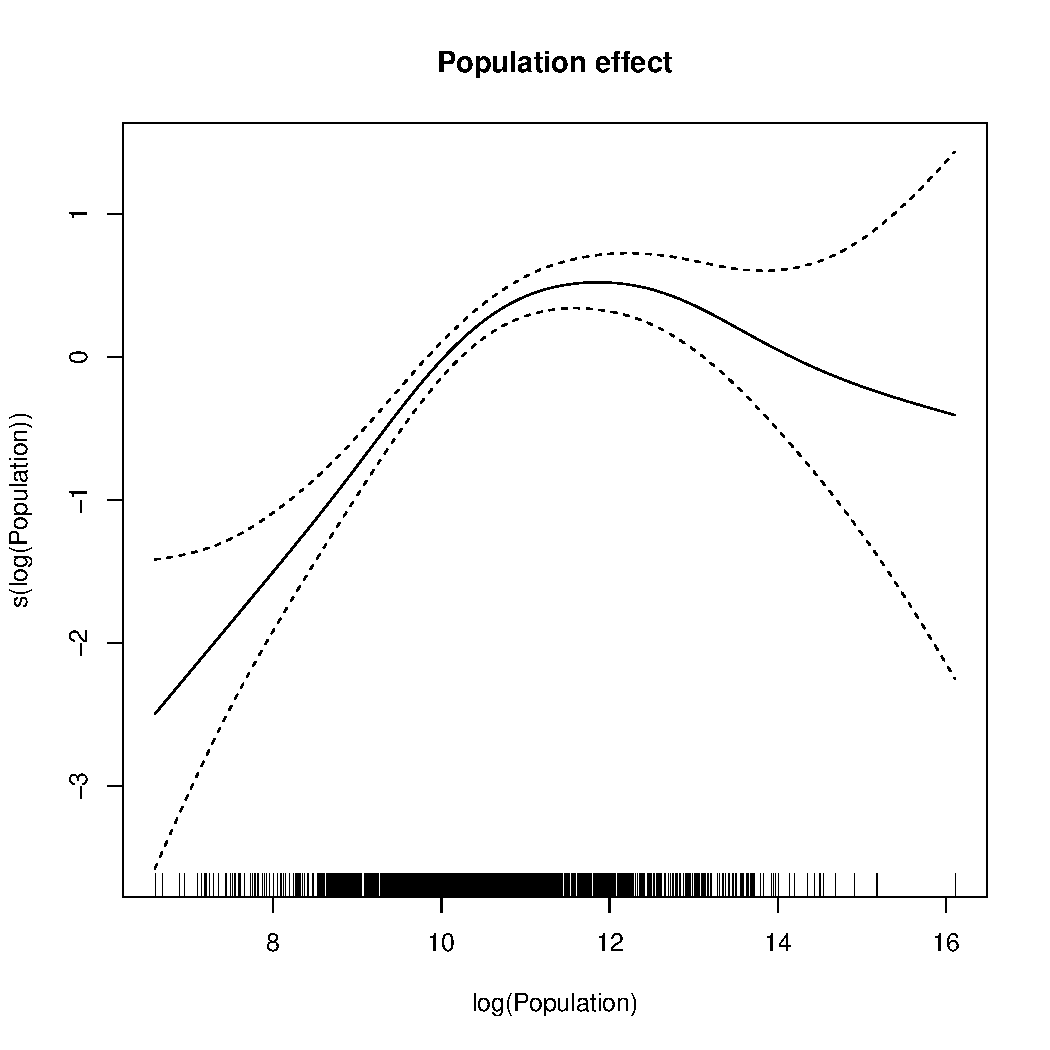
\includegraphics[width=\textwidth]{population_effect.pdf}
  \caption{Effect of population.}
  \label{fig:sub1}
\end{subfigure}%
\begin{subfigure}{.6\textwidth}
  \centering
  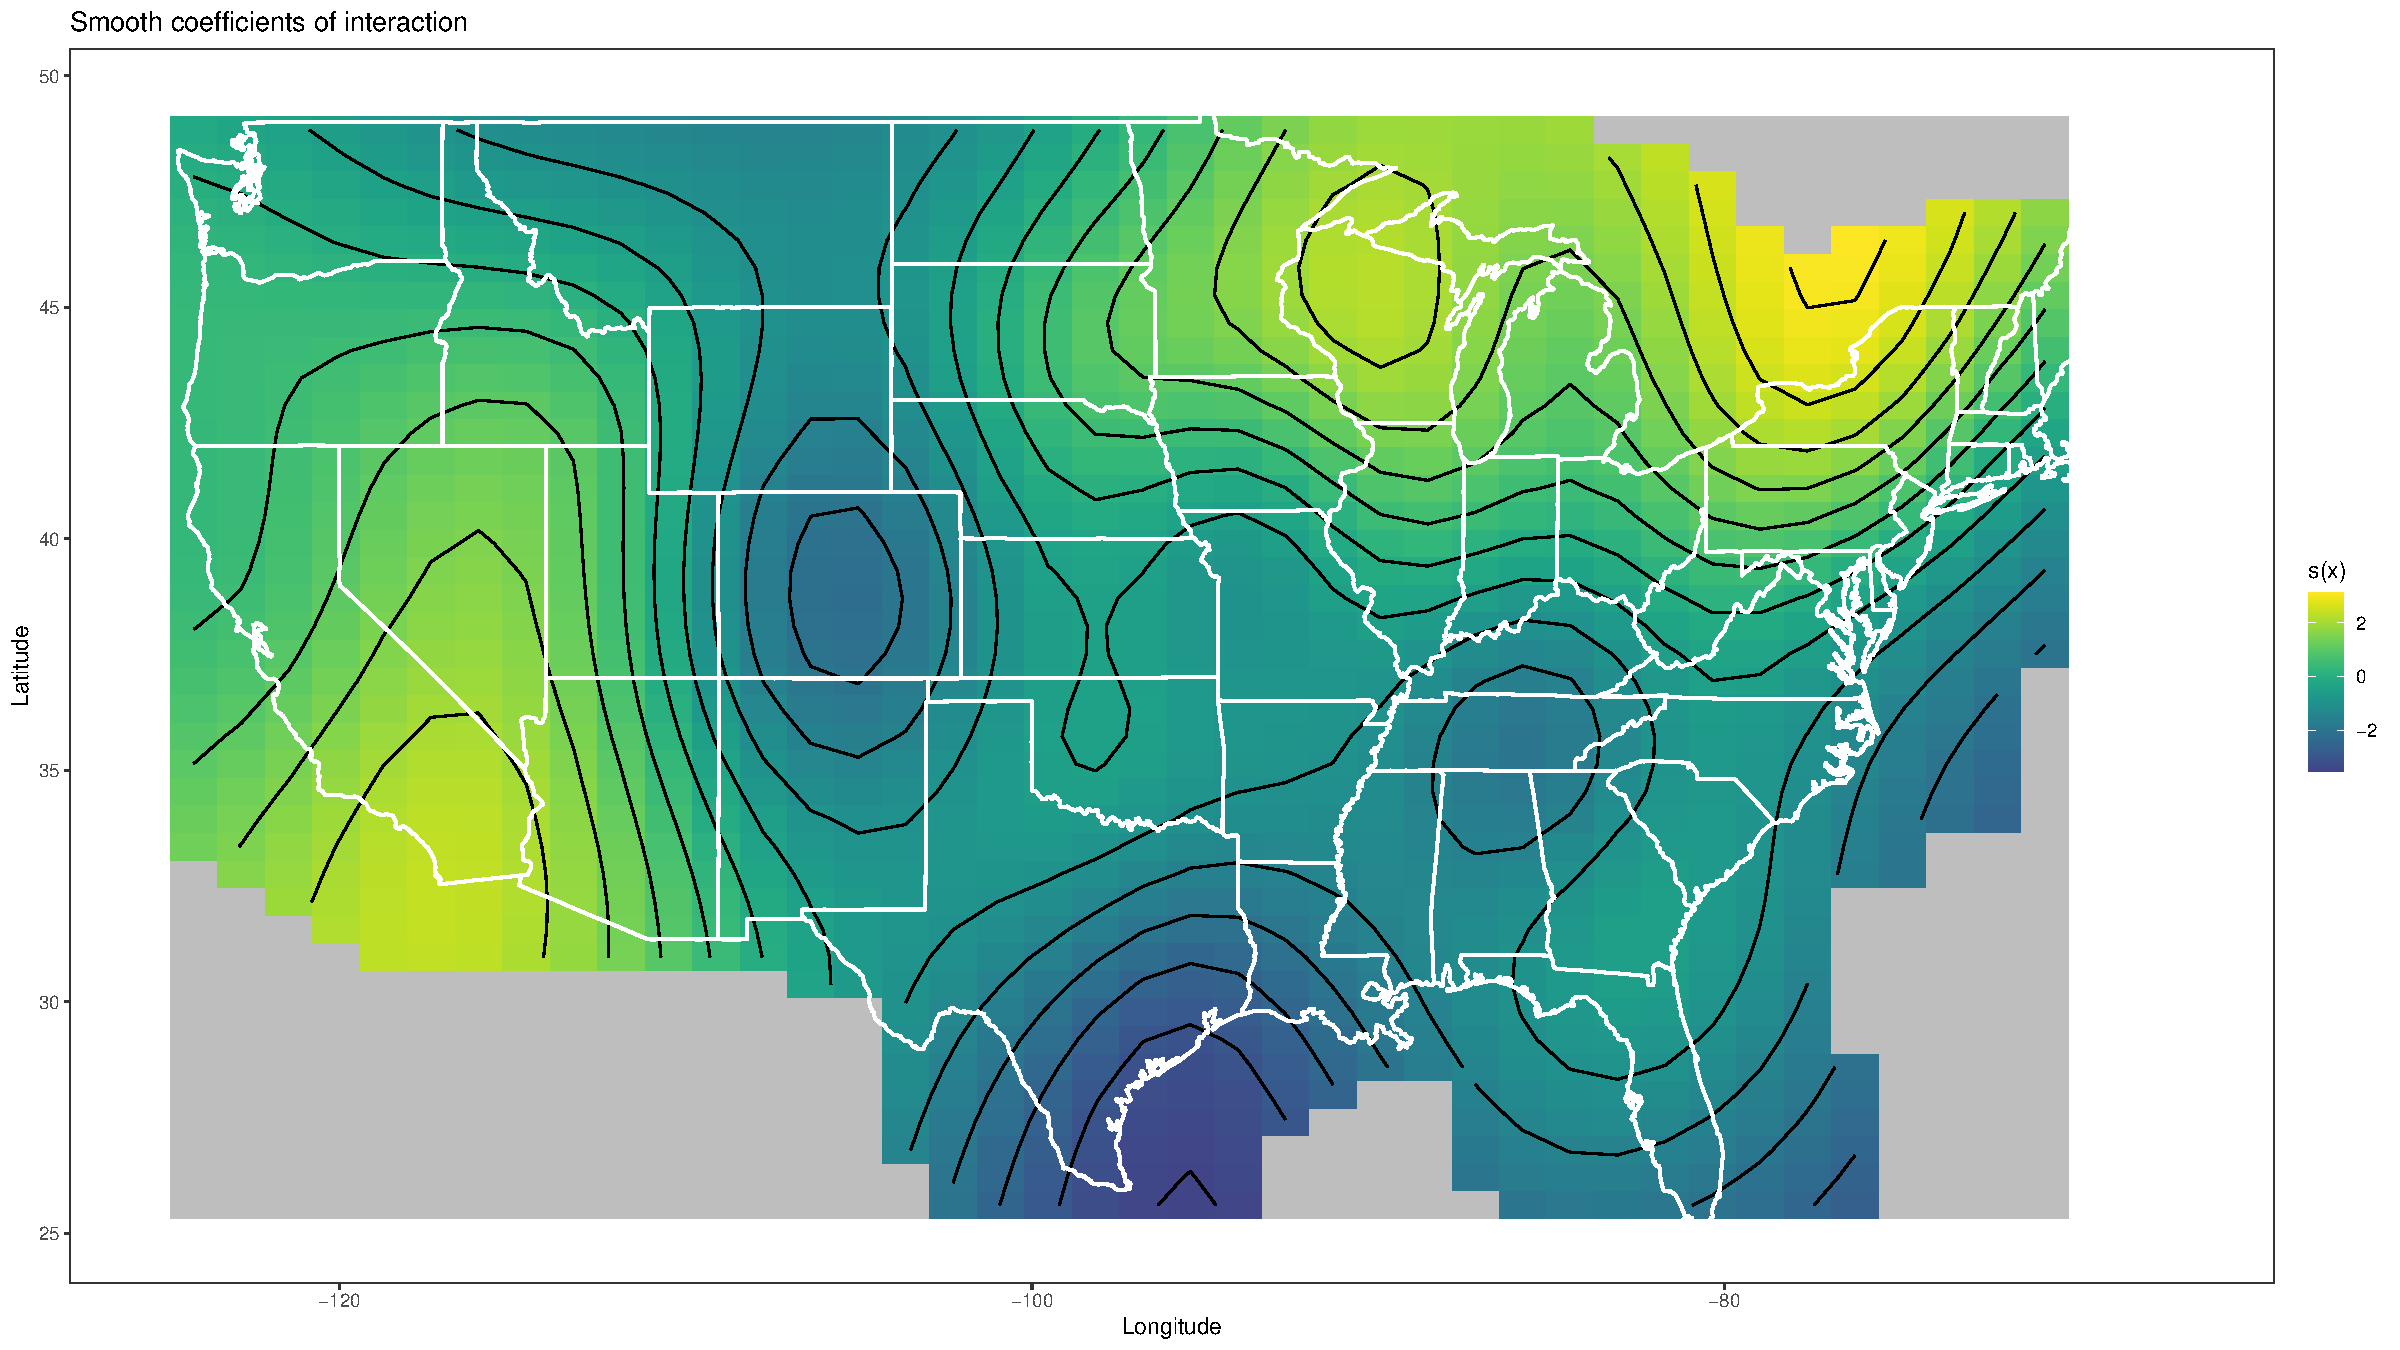
\includegraphics[width=\textwidth]{model2_coeff.pdf}
  \caption{Effect of latitude and longitude.}
  \label{fig:sub2}
\end{subfigure}
\caption{Effect of the coefficients in \ref{eq:model2_spatial}.}
\label{fig:coefficients_model2_spatial}
\end{figure}

%



\subsection{Consumption analysis with Bayesian Nonparametric Clustering}

The Dirichlet Process (DP) is a powerful tool in Bayesian nonparametric statistics that can be used for clustering functional data.
The cluster assignments and the parameters of the likelihood model are inferred using Markov Chain Monte Carlo (MCMC) sampling. The resulting samples from the posterior distribution provide a probabilistic clustering of the functional data.

Following this idea, we proceeded to implement a Nonparametric Bayesian clustering on the functional data describing the consumption of dairy in the last forty years.
\fg{0.6}{functional-consumption-exploratory-1.pdf}
In model \eqref{eq:bnp}, $\mathbf{y}_i=(y_{i 1},\ldots,y_{i T})$ represents the consumption of dairy $i$ at time $t$, $\mathbf{Z}$ and $\mathbf{X}$ are design matrices and $\boldsymbol{\alpha}_i$ and $\boldsymbol{\beta}_i$ are covariates of the linear model and take into account respectively the level of the time series and its trend. The $\boldsymbol{\theta}_i=(\theta_{i 1},\ldots,\theta_{i T})$ are described as an auto-regressive process of order 1 to take into consideration the effect of time. The clustering is performed only on the $\gamma_i = \left(\boldsymbol{\beta}_i, \boldsymbol{\theta}_i\right)$, in order to consider only the trend and the persistence of the time series. To perform such clustering a DP is set as prior for the distribution of the parameters $\gamma_i$.

\begin{equation}
    \label{eq:bnp}
    \begin{aligned}
    \mathbf{y}_i & =\mathbf{Z} \boldsymbol{\alpha}_i+\mathbf{X} \boldsymbol{\beta}_i+\boldsymbol{\theta}_i+\boldsymbol{\epsilon}_i, \quad i=1,2, \ldots, n \\
    \theta_{i t} & =\rho \theta_{i, t-1}+\nu_{i t} \quad \text{with }\nu_{i t}\sim \mathcal{N}(0, \sigma_{\theta}^2)\\
    \gamma_i &= \left(\boldsymbol{\beta}_i, \boldsymbol{\theta}_i\right) \\
    \gamma_i \mid G & \stackrel{\text{iid}}{\sim} G, \quad i=1,2, \ldots, n \\
    G & \sim \mathcal{DP}\left(a, b, G_0\right)
    \end{aligned}
\end{equation}

Using the R package \texttt{BNPTSclust} \cite{Nieto2014Bayesian}, implementing the above model, six clusters are obtained, three of which non-singletons.
Plotting them with their functional medians, we can instantly notice that the first cluster contains the dairy with an increasing trend over the years, the second the ones with decreasing consumption, and the third the cheese and kinds of milk with an oscillating behaviour.

\fg{0.9}{functional-bayesian-clustering-depth-median-1.pdf}

None of the 3 clusters has outliers.


\fg[Outliergram of Cluster 1.]{0.7}{functional-outliergram-1.pdf}
\fg[Outliergram of Cluster 2.]{0.7}{functional-outliergram-2.pdf}
\fg[Outliergram of Cluster 3.]{0.7}{functional-outliergram-3.pdf}

\subsubsection{Cluster analysis}

To be able to suggest to a stakeholder which dairy is more convenient to invest in, it is necessary to understand which dairy had an increase in consumption in the last years and most importantly why.

The results from the clustering are shown in Table \ref{tab:cluster}.

\begin{table}[htpb]
    \centering
    \small\setlength{\tabcolsep}{1pt}
    \begin{minipage}[t]{.33\linewidth}
        \centering
        %\caption{First Table}
        %\label{tab:first_table}
        \medskip
        \begin{tabular}{l}
            \toprule
            Cluster 1\\
            \midrule
            Cheddar\\
            American\_Other\\
            Mozzarella\\
            Italian\_other\\
            Muenster\\
            Cream\_and\_Neufchatel\\
            Other\_Dairy\_Cheese\\
            fluid\_yogurt\\
            butter\\
            cheese\_american\\
            cheese\_other\\
            evap\_cnd\_bulk\_and\_can\_skim\_milk\\
            dry\_buttermilk\\
            \bottomrule
        \end{tabular}
    \end{minipage}\hfill
    \begin{minipage}[t]{.3\linewidth}
        \centering
        %\caption{Second Table}
        %\label{tab:second_table}
        \medskip
        \begin{tabular}{l}
            \toprule
            Cluster 2\\
            \midrule
            Swiss\\
            Brick\\
            fluid\_milk\\
            cheese\_cottage\\
            evap\_cnd\_canned\_whole\_milk\\
            evap\_cnd\_bulk\_whole\_milk\\
            frozen\_ice\_cream\_regular\\
            frozen\_sherbet\\
            \bottomrule 
        \end{tabular}
    \end{minipage}\hfill
    \begin{minipage}[t]{.3\linewidth}
        \centering
        %\caption{Third Table}
        %\label{tab:third_table}
        \medskip
        \begin{tabular}{l}
            \toprule
            Cluster 3\\
            \midrule
            Foods\_and\_spreads\\
            frozen\_other\\
            dry\_whole\_milk\\
            dry\_whey\\
            \bottomrule                      
        \end{tabular}
    \end{minipage} 
    \caption{The 3 clusters of cheese types obtained.}
    \label{tab:cluster}
\end{table}


The first thing we can notice is how the consumption of fluid milk is decreased in the last forty years. Many factors contribute to declining fluid cow's milk consumption, including demographic and generational changes in the U.S. population. Younger generations who grew up drinking less milk as children appear to consume less at all ages.

Another cause can be found in the competition from other beverages—especially carbonated soft drinks, fruit juices, and bottled water—which is likely contributing to the changes in the frequency of fluid milk consumption \cite{Trends_chees}. In addition, substitutes for cow's milk (including nut milk, coconut milk, and soy milk) have provided alternatives for consumers.

Moreover, it's worth mentioning the decline in the consumption of ice cream contrasted with the increase in fluid yogurt. These differences across generations reflect in part their unique eating choices as children. Every decade brings a wider selection of dessert choices at supermarkets, restaurants, and other food outlets.

To conclude we can notice how, over the last four decades, Americans have increased their consumption of Italian varieties of cheese such as mozzarella, parmesan, and provolone \cite{Trends_chees}. The inclusion of cheese in time-saving convenience foods and in commercially manufactured foods such as frozen pizza and pre-packaged cheese slices, such as cheddar, has made increased the consumption of these varieties of dairy.




\section{Conclusions}

The results of this analysis provide valuable insights into the trends and patterns in the US dairy industry, which can inform decision-making and planning for both producers and consumers. Overall, this study provides a comprehensive overview of the US dairy industry and highlights its importance to the economy and society.

In terms of a pricing strategy, we obtained a flexible way of predicting an interval based on production factors.

For what concerns the choice of which product to produce, the Bayesian clustering showed that it's reasonable to invest, in the short term, in the varieties which have seen an increase in their consumption over the last few years if a conservative strategy is to be pursued. The best types of dairy in which to invest now are the Italian varieties of cheese and the ones used in commercially manufactured foods. While a more aggressive one would be to invest in the third cluster we found, which highlights a slight increase in the last years. 

Thanks to the spatial analysis we were able to get a prediction for the number of sales for all counties in Utah, establishing which are the ones with a higher demand to focus deliveries. In a possible future work, we could find a way to relate this quantity to the amount of milk to produce.